% !TeX root = ../thuthesis-example.tex

\chapter{go-ethereum的部分源码解读}

\section{整体结构}

go-ethereum的代码结构非常清晰,整个代码库主要分为以下几个部分:

\begin{itemize}
    \item accounts:这是管理以太坊账户的代码,包括账户管理、加密和解密、签名和验证等。
    \item cmd: 包含所有go-ethereum的命令行工具,如geth、abigen、bootnode等。
    \item core: 核心代码,包括区块链数据结构、区块链的实现、账户管理、交易执行等。
    \item crypto: 加密相关的代码,如私钥生成、签名等。
    \item consensus:这是区块链共识算法的实现,包括PoW(Proof of Work)、PoA、Ethash等。
    \item eth:以太坊网络协议的实现,包括区块同步、交易广播、状态传播和客户端协议等。
    \item internal:包含整个项目中使用的内部包。
    \item miner: 包含了以太坊矿工相关的代码,如挖矿、打包交易、广播区块等。
    \item node: 包含了以太坊节点相关的代码,如节点的启动、关闭、管理等。
    \item p2p: 网络层的实现,用于节点之间的通信。
    \item params: 包含了以太坊的参数配置,如区块链难度、网络ID、区块奖励等。
    \item storage:包含了以太坊的存储实现,如LevelDB等。
    \item rpc: 实现了以太坊的JSON-RPC API、WebSocket和IPC等。
    \item whisper: 实现了以太坊的whisper协议,用于点对点的消息传递,实现安全、私密的通信。
    \item trie: 包含了以太坊中使用的Merkle Patricia Trie数据结构相关的代码,如节点的添加、删除、查找等。
\end{itemize}

\section{部分核心源码的功能介绍}

由于我的实验目标与跨链与转账有关,故重点研究了树状区块链的结构,以及转账操作中涉及的代码内容。具体的代码注释已存入了我的毕设仓库当中。

图\ref{fig:树状区块链内部结构属性示意图}是树状区块链的内部结构属性示意图,展示了树状区块链的存储的各种属性,结合此图着重研究了区块链的区域索引的实现,树状多链结构的实现,区块汇总的实现以及跨链资产转移功能的实现。

\begin{figure}
	\centering
	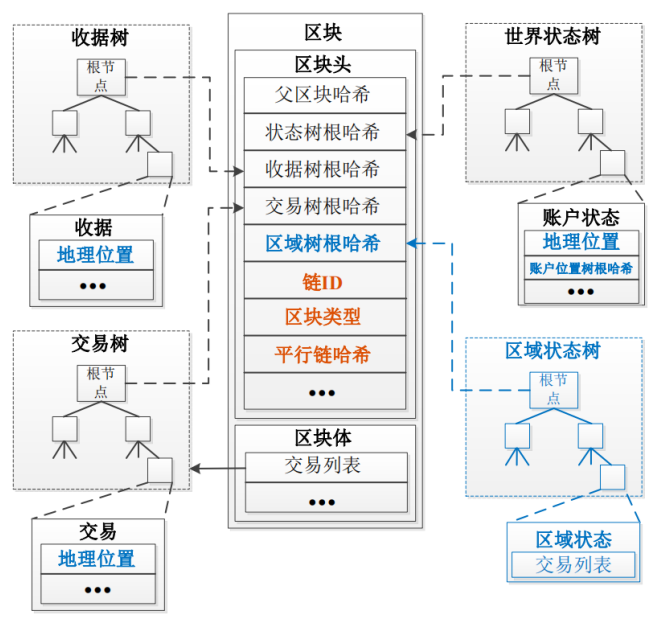
\includegraphics[width=0.6\textwidth]{figures/树状区块链结构属性示意图.png}
	\caption{树状区块链内部结构属性示意图}
	\label{fig:树状区块链内部结构属性示意图}
\end{figure}

\subsection{针对区域索引的说明}

首先是对创世块增加position的地理位置属性,创世块写入数据库并存储,实现存储创世块中的账户位置。

其次,对于account账户添加position的地理位置属性,同时实现获取账户位置的函数接口GetPosition,根据账户位置的hash值添加账户位置树;对于transaction交易添加position的地理位置属性。

实现并添加区域状态树,添加区域状态数据库,缓存区域状态,在miner中添加区域状态信息。区域状态树用于记录地理区块内的数据,便于地理信息的查询与相关数据的校验。

\subsection{针对树状多链的说明}

\begin{figure}
	\centering
	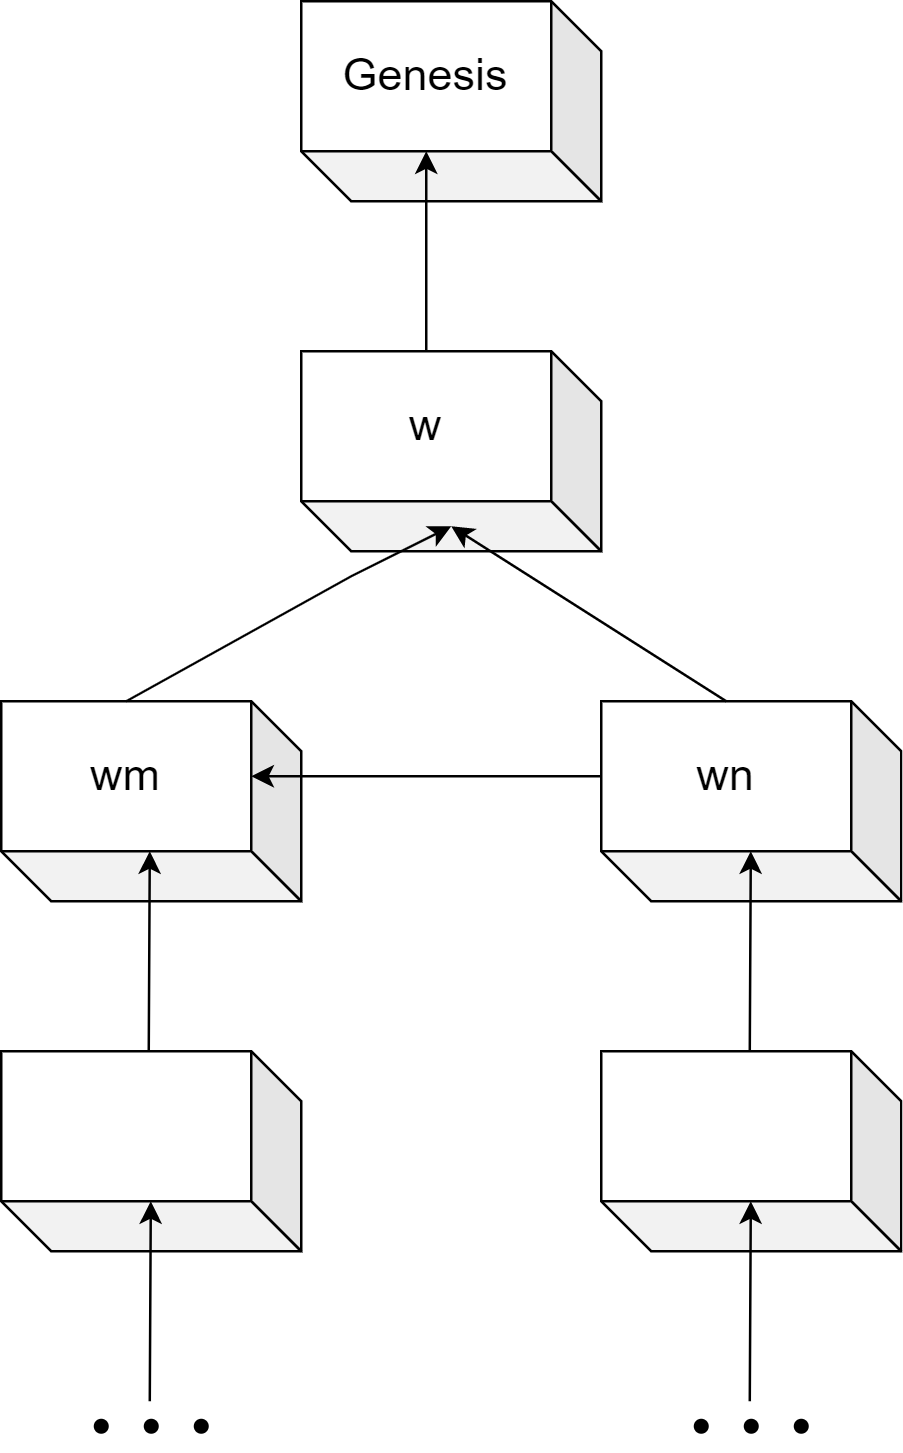
\includegraphics[width=0.4\textwidth]{figures/多链结构.png}
	\caption{树状结构}
	\label{fig:树状结构}
\end{figure}

将原本的单链结构变为多链结构,落实到代码中,添加了区块链内的链ID(chainID),区块类型(blockType)和平行链哈希(parallel Hash)。如图\ref{fig:树状区块链内部结构属性示意图}和图\ref{fig:树状结构}所示,链 ID(chainID)的作用是区分来自不同区块链的区块。区块类型是指支持区域索引的树状区块链将区块分为了三种区块:创世块、分支区块、普通区块。该属性即是指对当前区块类型的划分。平行链哈希则是分支区块不仅仅需要用父链指针指向自己的上层区块,同时还需要用一个平行链指针指向跟自己拥有相同父区块且Geohash编码的前n-1位相同的已产生的同层级分支区块。

\subsection{针对区块汇总的说明}

\begin{figure}
	\centering
	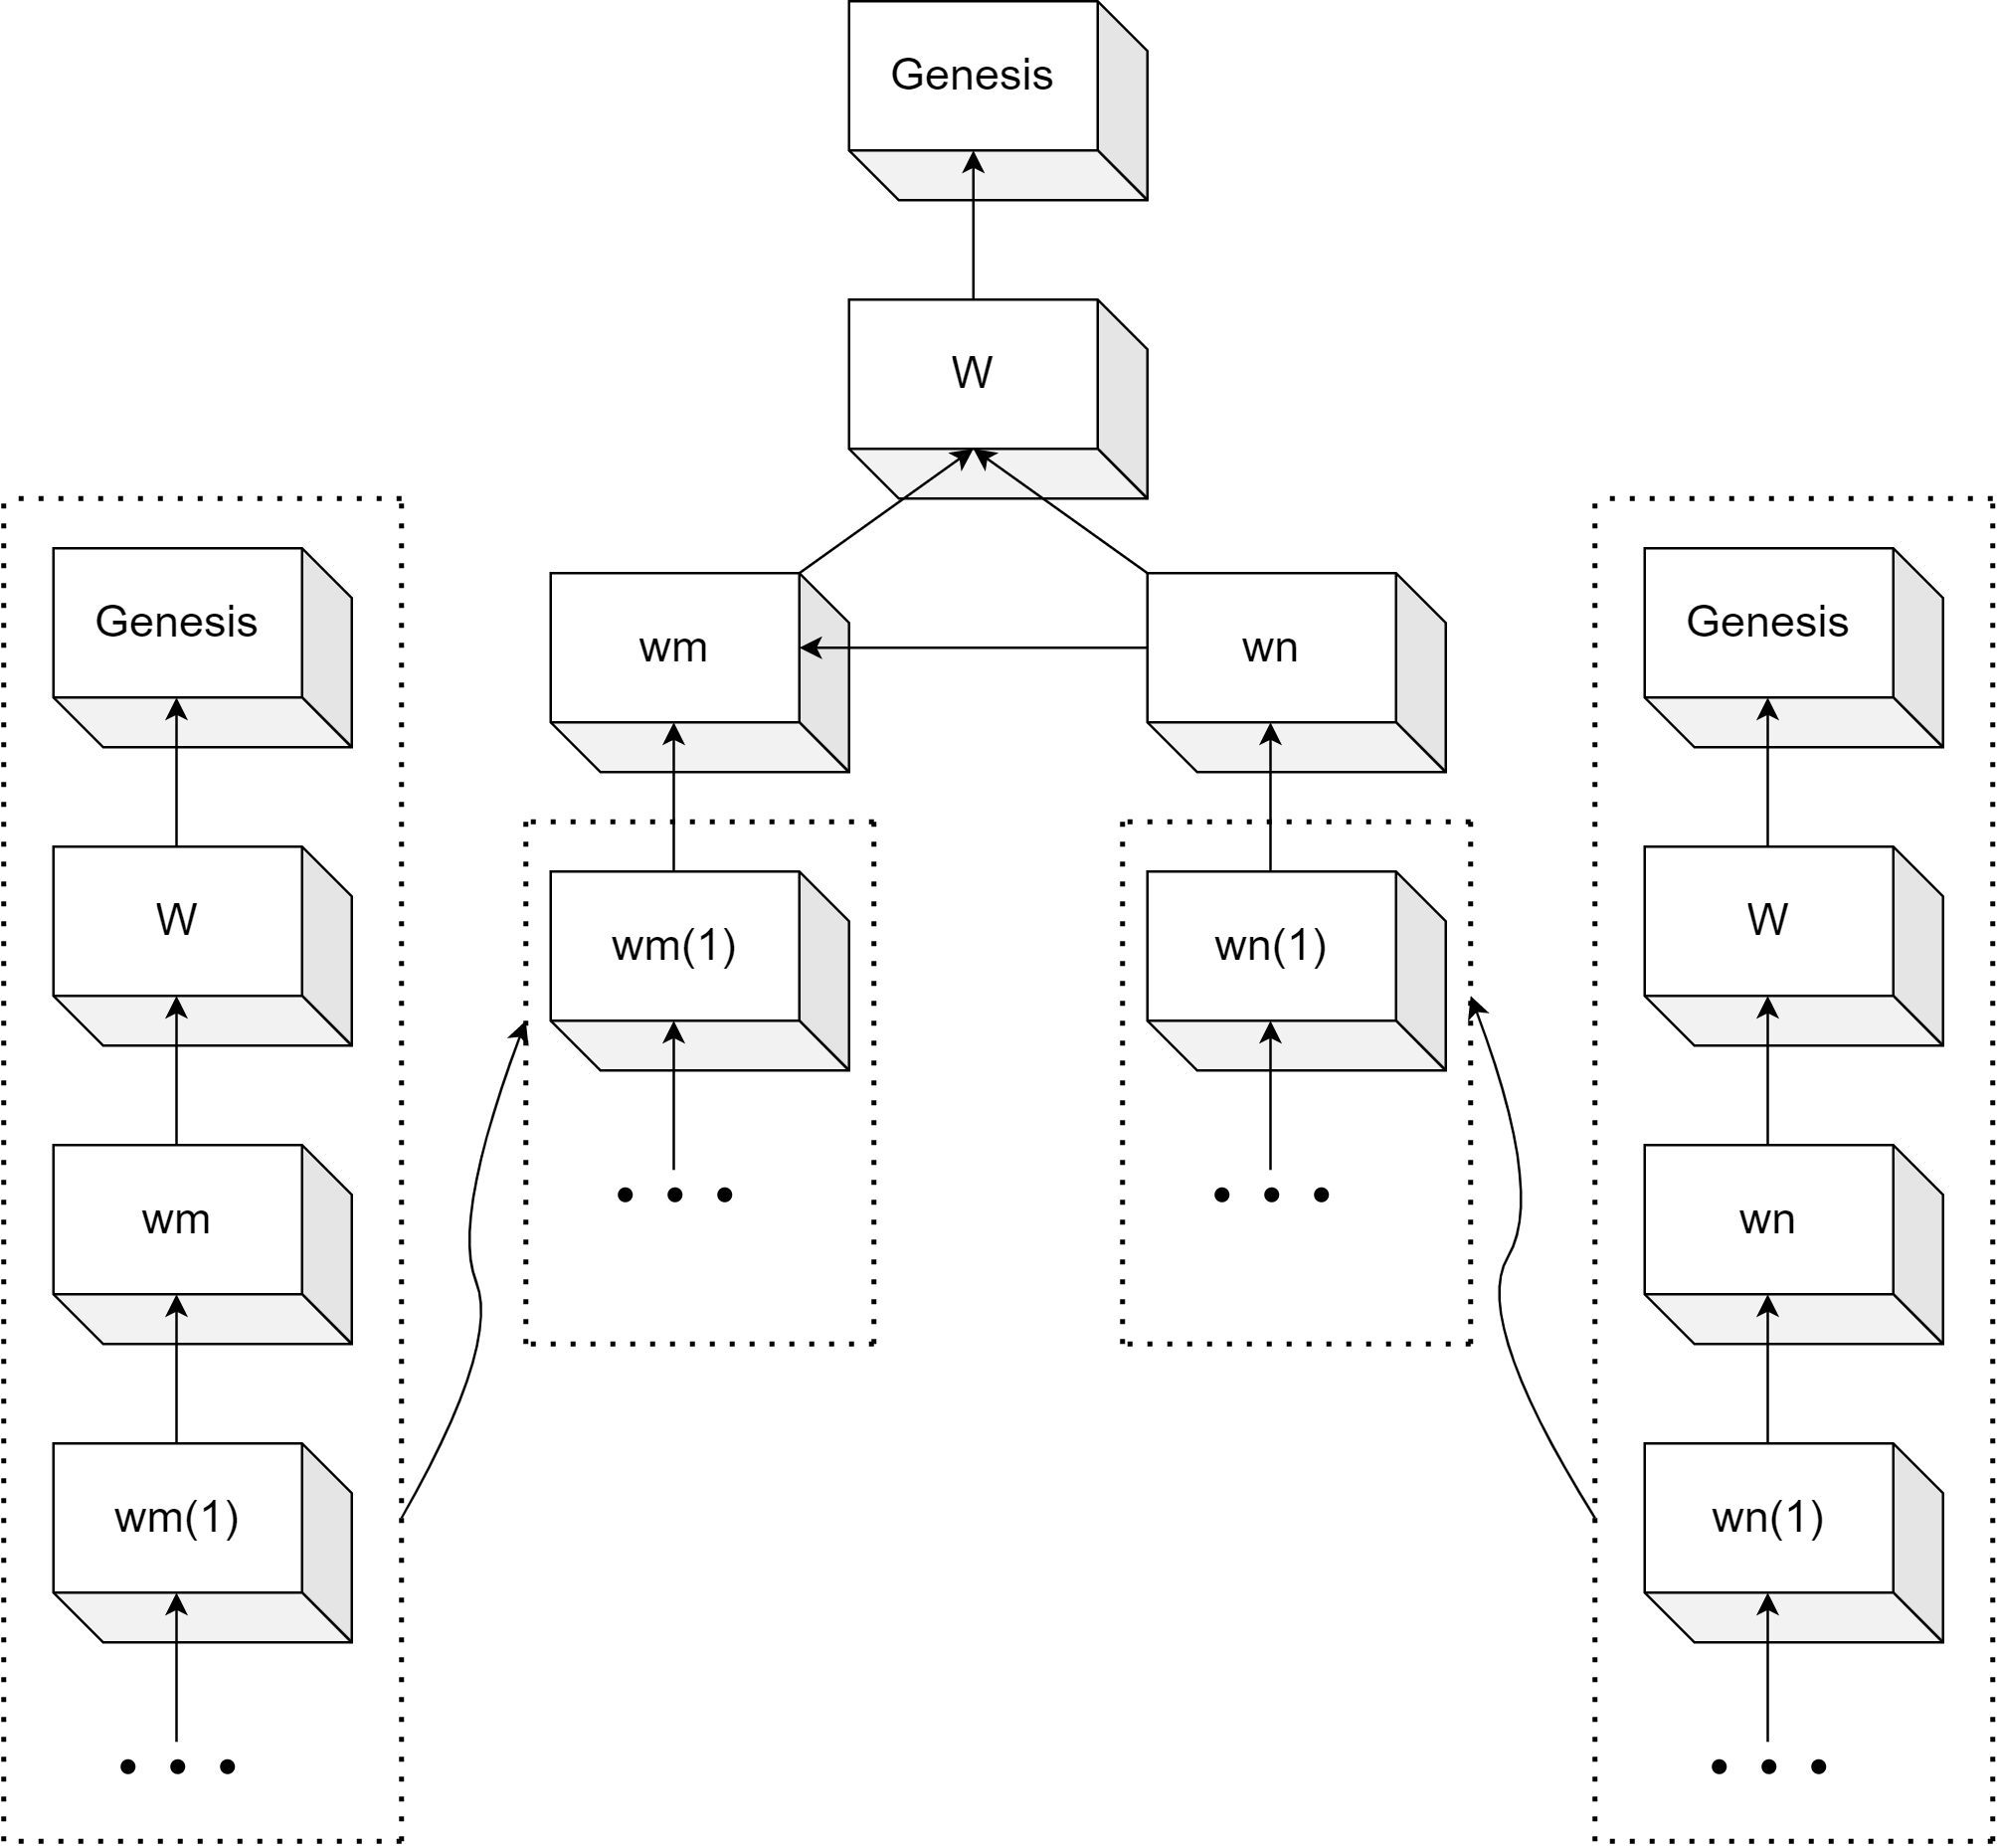
\includegraphics[width=0.8\textwidth]{figures/区块汇总过程示意图.png}
	\caption{区块汇总过程示意图}
	\label{fig:区块汇总过程示意图}
\end{figure}

节点中记录分支区块,并增加同步分支区块,区块汇总的方式,分支节点可以生成分支区块,分支区块写入区块链后,会根据regionid同步区块。

图\ref{fig:区块汇总过程示意图}为区块汇总过程示意图。分支节点在进行区块汇总时,按照子链地理区域独立汇总,最终可以将各子链中需要同步的区块都同步到分支区块中的对应的区域的分支上,此外,同步后的区块的内容以及其排列顺序都与待汇总子链相同,保证了各子链中交易顺序的不变性。

\subsection{针对资产转移的说明}

\begin{figure}
	\centering
	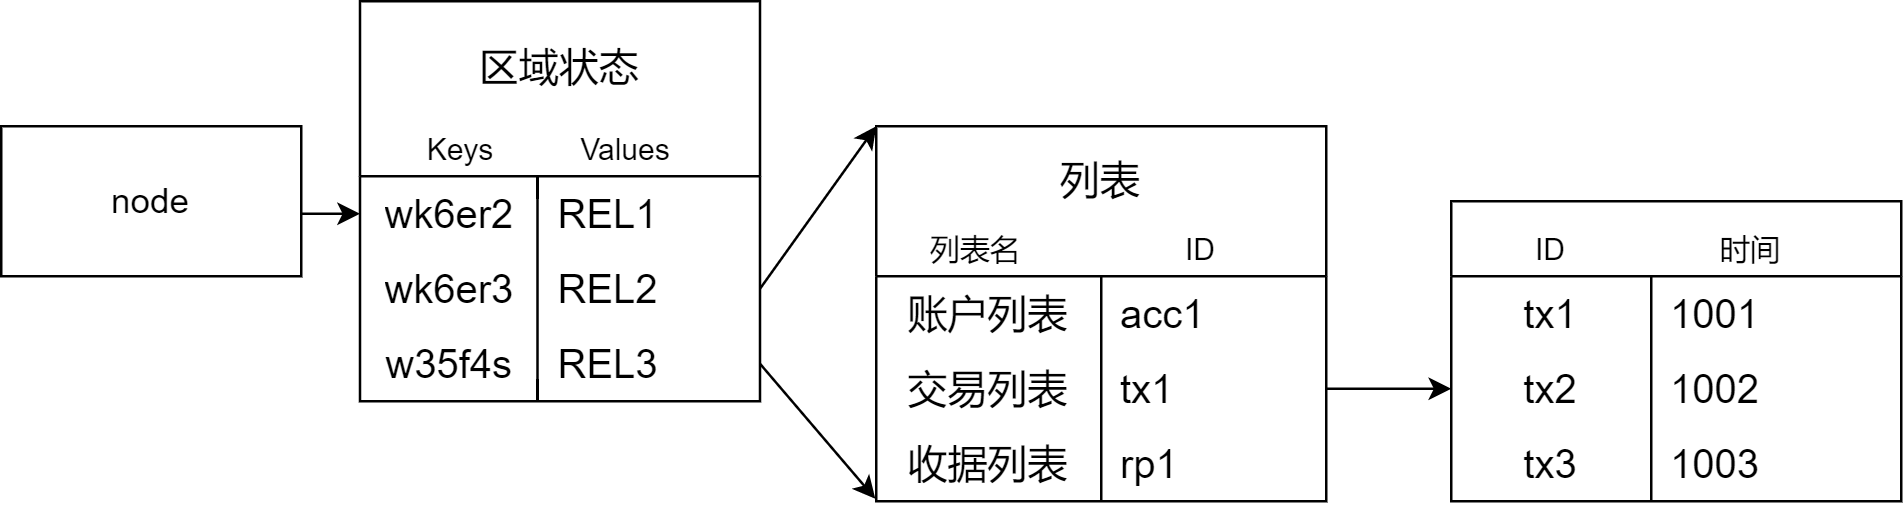
\includegraphics[width=\textwidth]{figures/交易列表.png}
	\caption{节点中资产转移列表相关结构}
	\label{fig:节点中资产转移列表相关结构}
\end{figure}

如图\ref{fig:节点中资产转移列表相关结构}所示,在分支节点中管理着资产转移交易列表,该列表结构中存储着子链发起的资产转移交易内容,此外对于添加进该列表的交易,代码还实现了交易的原子性操作。

资产转移交易被定义为特殊的交易类型,其设定为不需要消耗gas,此外,相较于传统交易,资产转移交易额外增加了一个自定义的txtype属性,列表中记录了该txtype属性以及对应的时间戳。

分支节点在同步区块时,若接受到含有txtype属性的交易,则判断此交易是否是资产转移交易,根据接收到的txtype值的不同进行后续的不同事件处理,包括目标链发起请求,来源链转出请求,目标链转入资金,来源链记录交易。

\section{本章小结}

本章对现有系统使用的树状区块链源码中的部分功能所涉及到的源码作了注释,详细说明在仓库中。

主要作用是方便后续工作者更好地理清代码逻辑,可以对整个系统的运作流程更为清晰。同时,也便于未来可能的对现有的底层源码的改进工作的进行。
